\documentclass[ignorenonframetext,xcolor=x11names]{beamer}

\input{../common.preamble.beamer.tex}

\title{Business 4720 - Class 23}

\subtitle{Legal Issues in Business Analytics}

\begin{document}

\begin{frame}{}
  \titlepage
  \footnotesize
  \input{../license.tex}
\end{frame}

\section{Introduction}

\begin{frame}{This Class}
\begin{block}{What You Will Learn:}
\begin{itemize}
  \item Torts 
  \item Contracts 
  \item Copyright 
  \item Web-sites 
  \item Privacy legislation (PIPEDA)
  \item Artifical intelligence and data act (AIDA, Bill C-27)
  \item European Union AI Act
\end{itemize}
\end{block}
\end{frame}

\begin{frame}{Torts}
\begin{block}{Review of Concepts}
  \begin{itemize}
     \item Civil wrong, other than breach of contract
     \item Vicarious liability for employees
     \item Compensatory and punitive damages, injunctions
  \end{itemize}
\end{block}
\end{frame}

\begin{frame}{Intentional Torts}
\begin{block}{''Invasion of Privacy''}
  \begin{itemize}
     \item Trespass (e.g. to collect image or other sensor data)
     \item Breach of confidence (e.g. unauthorized use of confidential information)
     \item Intrusion on seclusion  (e.g. employees inappropriately using data access)
     \item Public disclosure of private facts
  \end{itemize}
\end{block}  
\begin{block}{Defenses}
  \begin{itemize}
     \item Consent
     \item Assumption of risk
     \item Contributory negligence
  \end{itemize}
\end{block}
\end{frame}

\begin{frame}{Negligence}
\begin{block}{Examples}
\begin{itemize}
  \item Data loss or breach
  \item Physical or economic loss due to advice based on analytics models
\end{itemize}
\end{block}

\begin{block}{Duty of Care}
  \begin{itemize}
    \item Reasonably foreseeable
    \item Affordable precautions
    \item Proximity of loss (incl. careless statements)
    \item Product liability (incl. data/information products)
  \end{itemize}
\end{block}
\begin{block}{Defenses}
  \begin{itemize}
     \item Asumption of risk
     \item Contributory negligence
  \end{itemize}
\end{block}
\end{frame}

\begin{frame}{Contracts} 
  \begin{block}{General Concepts}
  \begin{itemize}
     \item Contract creation and acceptance of offers
     \item UECA and provincial electronic commerce acts
     \begin{itemize}
        \item Specifies communication (sending, receiving) of offers and acceptance
     \end{itemize}
     \item Consideration, privity, and assignment
     \item Terms, misrepresentation (negligence, fraud)
     \item Compensation or rescission (how?), and obstacles
     \item Exclusion, limitation, and waiver clauses
  \end{itemize}
  \end{block}
\end{frame}

\begin{frame}{Contracts}
  \begin{block}{Examples In Business Analytics}
  \begin{itemize}
     \item Purchase or sale of data
     \item Collection or creation of data
     \item Licensing of data
     \item Data processing and manipulation (e.g. data cleaning, anonymization, etc)
     \item Provide or access/use analytics services
   \end{itemize}
   \end{block}
   \begin{block}{Specify}
   \begin{itemize}
      \item What is being purchased (e.g. copyright (assignment), licence, or analytics service)?
      \item What is the required quality and how is it measured?
   \end{itemize}
   \end{block}
\end{frame}

\begin{frame}{Licences}
  \begin{block}{Permission to Use or Do Something}
  \begin{itemize}
     \item Exclusive, sole, or non-exclusive (ordinary)
     \item Revocable or irrevocable
     \item Transferrable or non-transferrable
     \item Sublicenseable or not sublicenseable
     \item Limited or unlimited (in time or geography)
     \item Permitted uses (granted rights)
     \item Requirements for use
     \item Warranties, explicit or implied
     \item Indemnification
  \end{itemize}
  \end{block}
\end{frame}

\begin{frame}{Copyrights}
  \begin{block}{What is copyrightable?}
  \begin{itemize}
     \item Non-trivial, original work
     \item Requiring \emph{skill and judgment}
     \item Data as compilation of facts?
     \item Copyrightable by transformation, curation, collection 
     \end{itemize}
  \end{block}
  \begin{block}{What are the copyrights?}
  \begin{itemize}
     \item Reproduction (copying), making available, adaptation, translation, etc.
     \item Is data ingestion into a prediction model reproduction, adaptation, or translation? (''temporary reproduction'')
  \end{itemize}
  \end{block}
\end{frame}

\begin{frame}{Websites}
  \begin{block}{Using Web Data}
  \begin{itemize}
     \item Terms of use 
     \item Automatic access (''bots'', ''crawlers'')
  \end{itemize}
  \end{block}
  \begin{block}{Robots files}
     \begin{itemize}
       \item Specify user agent (''User-agent'')
       \begin{itemize}
          \item ''Googlebot'', ''Bingbot'', ''Googlebot-Image'', \ldots
       \end{itemize}
       \item Specify prohibited files or folders (all others allowed)
       \item Specify allowed files or folders (all others prohibited)
       \item Specify crawl frequency (''Crawl-delay'')
       \item Specify no search indexing (''Noindex'')
     \end{itemize}
  \end{block}
\end{frame}

\begin{frame}[fragile]{Example Robots File}
\begin{textcode}
# robots.txt file for YouTube
# Created in the distant future (the year 2000) after
# the robotic uprising of the mid 90's which wiped 
# out all humans.

User-agent: Mediapartners-Google*
Disallow:

User-agent: *
Disallow: /api/
Disallow: /comment
Disallow: /feeds/videos.xml

Disallow: /watch_popup
Disallow: /watch_queue_ajax
Disallow: /youtubei/
\end{textcode}
\scriptsize Source: \url{youtube.com/robots.txt}
\end{frame}

\begin{frame}{Hands-On Exercise}
\begin{columns}
\begin{column}{0.2\textwidth}
\href{https://commons.wikimedia.org/wiki/File:Emojione_BW_1F44B.svg}{
\includegraphics[width=\textwidth]{hand.png}}
\end{column}
\begin{column}{0.8\textwidth}
Identify the robots.txt file of your university web site.
\begin{itemize}
  \item Are there portions of the site a crawler bot is not permitted? Why might this be?
  \item Are there different directives for different crawlers?
  \item Are there limits on crawl frequency?
\end{itemize}
\end{column}
\end{columns}
\end{frame}


\begin{frame}{Privacy Legislation}
  \begin{itemize}
     \item Personal Information Protection and Electronic Documents Act (PIPEDA) (federal)
     \item Applies to commercial activity in all Canadian provinces
     \item Except for activity solely within provinces that have ''substantially similar'' legislation (BC, ON)
     \item Does not apply to federal government, covered by Privacy Act and Access to Information Acts
     \item Does not apply to provincial government (e.g. Newfoundland Access to Information and Protection of Privacy Act (ATIPPA))
  \end{itemize}
\begin{itemize}
   \item Office of the Privacy Commissioner of Canada (OPC)
   \begin{itemize}
      \item Investigate complaints
      \item Report with recommendation but no enforcement powers
      \item Federal Court
   \end{itemize}
\end{itemize}
\end{frame}

\begin{frame}{PIPEDA}
  \begin{block}{Personal Information}
    \begin{itemize}
       \item Name, age, weight, height
       \item Medical information, e.g. medical records
       \item Financial information, e.g. income, purchases, \ldots
       \item Race and ethnicity, marital status and religion
       \item Biometrics, such as DNA and fingerprints
       \item Address and communication info (email, phone \#, \ldots)
       \item Eduction, such as transcripts and grades
       \item Employment information and employment records
       \item Opinions and comments
    \end{itemize} 
  \end{block}
\end{frame}

\begin{frame}{PIPEDA}
\begin{block}{Fair Information Principles}
\begin{enumerate}
   \item Be accountable
   \item Identify the purpose
   \item Obtain valid, informed consent
   \item Limit collection
   \item Limit use, disclosure and retention
   \item Be accurate
   \item Use appropriate safeguards
   \item Be open
   \item Give individuals access
   \item Challenging compliance
\end{enumerate}
\end{block}
\end{frame}

\begin{frame}{PIPEDA}
\begin{itemize}
   \item Mandatory breach reporting
   \item Complaint process through the OPC
   \item Authority to audit
\end{itemize}
\begin{block}{Sources and Further Information}
\begin{itemize}
   \item \href{https://www.priv.gc.ca/media/2038/guide_org_e.pdf}{Privacy Guide for Businesses (OPC)}
   \item \href{https://www.priv.gc.ca/en/privacy-topics/privacy-laws-in-canada/the-personal-information-protection-and-electronic-documents-act-pipeda/p_principle/}{PIPEDA fair information principles (OPC)}
\end{itemize}
\end{block}
\end{frame}

\begin{frame}{PIPEDA -- 1. Accountability}
\begin{block}{Requirements}
  \begin{itemize}
     \item Comply with all 10 principles
     \item Appoint person responsible for compliance (privacy officer)
     \item Define reporting mechanisms to/from this person or office
     \item Protect all personal information, incl. that transferred to 3rd parties and agents
     \item Develop and implement policies and procedures for compliance
  \end{itemize}
\end{block}

\vspace{\baselineskip}
\scriptsize \textbf{Source:} \href{https://www.priv.gc.ca/en/privacy-topics/privacy-laws-in-canada/the-personal-information-protection-and-electronic-documents-act-pipeda/p_principle/principles/p_accountability/}{PIPEDA Fair Information Principle 1 -- Accountability (OPC)}
\end{frame}

\begin{frame}{Hands-On Exercise}
\begin{columns}
\begin{column}{0.2\textwidth}
\href{https://commons.wikimedia.org/wiki/File:Emojione_BW_1F44B.svg}{
\includegraphics[width=\textwidth]{hand.png}}
\end{column}
\begin{column}{0.8\textwidth}

Identify the privacy policy of your bank or communications provider or other large organization you regularly deal with. 
\begin{itemize}
  \item Who is the responsible person?
  \item Who do they report to?
  \item How can you contact them?
\end{itemize}
\end{column}
\end{columns}
\end{frame}


\begin{frame}{PIPEDA -- 1. Accountability \small (Building Blocks)}
   \begin{itemize}
      \item \textbf{Information inventory}, incl. sensitivity evaluation
      \item \textbf{Policies} for
         \begin{itemize}
           \item Collection, use and disclosure (incl. consent \& notification)
           \item Access to and correction of information
           \item Retention and disposal
           \item Administrative, physical and technological security controls and access privileges
           \item Challenging compliance
         \end{itemize}
      \item \textbf{Risk and threat assessment} for all operations (esp. involving 3rd parties outside Canada)
      \item \textbf{Privacy training and education} for all employees
      \item \textbf{Breach and incident management} protocols
      \item \textbf{Manage external service providers} with access to data (e.g. contractual provisions, training and education, audits)
      \item \textbf{External communication} procedures (notification, access/contact means, etc.)
   \end{itemize}

\vspace{.5\baselineskip}
\scriptsize \textbf{Source:} \href{https://www.priv.gc.ca/en/privacy-topics/privacy-laws-in-canada/the-personal-information-protection-and-electronic-documents-act-pipeda/pipeda-compliance-help/pipeda-compliance-and-training-tools/gl_acc_201204/}{Getting accountability right with a privacy management program (OPC)}
\end{frame}

\begin{frame}{PIPEDA -- 1. Accountability \small (Ongoing Assessment and Revision)}
\begin{itemize}
  \item Oversight plan for monitoring privacy management effectiveness and compliance
  \item Periodically review and revise plan
  \item Monitor ongoing processes:
  \begin{itemize}
     \item Are controls effective?
     \item Do controls reflect latest OPC or industry guideslines?
     \item Are new services being offered that involve increased collection, use, or disclosure?
     \item Is training being delivered and effective?
     \item Are policies known and followed?
  \end{itemize}
  \item Document compliance for audits and investigations
\end{itemize}

\vspace{\baselineskip}
\scriptsize \textbf{Source:} \href{https://www.priv.gc.ca/en/privacy-topics/privacy-laws-in-canada/the-personal-information-protection-and-electronic-documents-act-pipeda/pipeda-compliance-help/pipeda-compliance-and-training-tools/gl_acc_201204/}{Getting accountability right with a privacy management program (OPC)}
\end{frame} 

\begin{frame}{PIPEDA -- Cross-Border Personal Data Processing}
\begin{itemize}
   \item The transferring organization remains accountable
   \item Contractually ensure generally equivalent protection
   \item Take all reasonable steps to protect data
   \begin{itemize}
      \item Contractual terms
      \item External party staff training
      \item External party security measures
      \item Audits and inspection
   \end{itemize}
   \item Be aware of legal requirements of the jurisdiction in which the third party processor operates, e.g. 
   \begin{itemize}
      \item Financial information disclosure requirements
      \item National security access to information
   \end{itemize}
\end{itemize}

\vspace{\baselineskip}
\scriptsize \textbf{Source:} \href{https://www.priv.gc.ca/en/privacy-topics/airports-and-borders/gl_dab_090127/}{Guidelines for processing personal data across borders (OPC)}
\end{frame}

\begin{frame}{PIPEDA -- 2. Identifying Purpose}
\begin{itemize}
   \item Ensure information is required for purpose
   \item Explain purpose when collecting information
   \item Maintain records for purpose and received consents
   \item Ensure purpose is reasonably and appropriately limited
\end{itemize}

\vspace{\baselineskip}
\scriptsize \textbf{Source:} \href{https://www.priv.gc.ca/en/privacy-topics/privacy-laws-in-canada/the-personal-information-protection-and-electronic-documents-act-pipeda/p_principle/principles/p_purposes/}{PIPDA Fair Information Principle 2 -- Identifying purposes (OPC)}
\end{frame}

\begin{frame}{PIPEDA -- 3. Consent}
\begin{itemize}
   \item Consent must be meaningful and valid
   \item Consent can be required only if necessary to fulfill a legitimate purpose
   \item Form of consent must take into account the sensitivity of information
   \item Individuals may withdraw consent at any time
\end{itemize}

\vspace{\baselineskip}
\scriptsize \textbf{Source:} \href{https://www.priv.gc.ca/en/privacy-topics/privacy-laws-in-canada/the-personal-information-protection-and-electronic-documents-act-pipeda/p_principle/principles/p_consent/}{PIPDA Fair Information Principle 3 -- Consent (OPC)}
\end{frame}

\begin{frame}{PIPEDA -- 3. Consent \small (Guidelines)}
\begin{itemize}
   \item Make privacy information clearly available: \emph{what} information is collected, \emph{who} is it shared with, \emph{for what} purpose, and what are the \emph{potential risks or harms}?
   \item Provide a clear choice
   \item Ensure the consent process is user friendly
   \item Allow individuals to withdraw consent
   \item Re-obtain consent when making significant changes to privacy practices
   \item Retain records to demonstrate compliance
\end{itemize}

\vspace{\baselineskip}
\scriptsize \textbf{Source:} \href{https://www.priv.gc.ca/en/privacy-topics/collecting-personal-information/consent/info_mc/}{Optaining meaningful consent infographic (OPC)}

\vspace{\baselineskip}
\scriptsize \textbf{Source:} \href{https://www.priv.gc.ca/en/privacy-topics/collecting-personal-information/consent/gl_omc_201805/}{Guidelines for obtaining meaningful consent (OPC)}
\end{frame}

\begin{frame}{PIPEDA -- 3. Consent \small (Interpretation)}
\begin{itemize}
   \item Consent is necessary, but not sufficient
   \item Purpose of collection must be ''reasonable''
   \begin{itemize}
   \item Information collection must serve real business interest
   \item Loss of privacy must be proportional to benefits gained
   \end{itemize}
\end{itemize}
\begin{block}{''No-Go Zones''}
\begin{itemize}
   \item Collection, use or disclosure that would be illegal
   \item Profiling or categorization that leads to unfair, unethical, or discriminatory treatment
   \item Collection, use or disclosure that is likely to cause significant harm
   \item Publishing information with intent to charge for removal
   \item Requiring social media passwords for employee screening
   \item Surveillance through an individual's own device
\end{itemize}
\end{block}

\vspace{.5\baselineskip}
\scriptsize \textbf{Source:} \href{https://www.priv.gc.ca/en/privacy-topics/collecting-personal-information/consent/gd_53_201805/}{Guidance on inappropriate data practices: Interpretation and application of subsection 5(3) (OPC)}
\end{frame}

\begin{frame}{PIPEDA -- 3. Consent \small (Example Decisions)}
\begin{itemize}
   \item Number of gym visits: Collection may be benign but disclosure to work team members may not be, requiring explicit consent
   \item Viewing of health-related websites is sensitive information.
   \item Email address may be sensitive if it indicates social connection.
   \item Palm-vein scanning is not sensitive if the scan is not retained and immediately transformed.
   \item Disclosure of sensitive financial information requires explicit consent, while disclosure of customer contact for financial marketing may only require opt-out consent.
   \item Purchasing habits are sensitive, require explicit consent
   \item Voice prints for computer authentication are not sensitive
   \item Non-users of social networking sites would not reasonably expect the use of their email addresses for creating links, requiring explicit consent.
\end{itemize}

\vspace{.5\baselineskip}
\scriptsize \textbf{Source:} \href{https://www.priv.gc.ca/en/privacy-topics/privacy-laws-in-canada/the-personal-information-protection-and-electronic-documents-act-pipeda/pipeda-compliance-help/pipeda-interpretation-bulletins/interpretations_07_consent/}{Interpretation Bulletin: Form of Consent (OPC)}
\end{frame}

\begin{frame}{PIPEDA -- 3. Consent \small (Implied Consent)}
\begin{itemize}
   \item In initiating a complaint procedure, medical information may be be disclosed to the defendant in order to defend themselves through implied consent.
   \item GPS location data may be collected by implied consent for the purposes of improving productivity, or protecting and managing company assets, but not for employee evaluation.
\end{itemize}

\scriptsize \textbf{Source:} \href{https://www.priv.gc.ca/en/privacy-topics/privacy-laws-in-canada/the-personal-information-protection-and-electronic-documents-act-pipeda/pipeda-compliance-help/pipeda-interpretation-bulletins/interpretations_07_consent/}{Interpretation Bulletin: Form of Consent (OPC)}
\end{frame}

\begin{frame}{PIPEDA -- 3. Consent \small (Conditions for Opt-out Consent)}
\begin{itemize}
   \item Information is non-sensitive in nature and in context.
   \item Information sharing is limited and well-defined
   \item Organization's purposes are limited and well-defined and clearly stated at time of collection
   \item Opportunity for opt-out offered at the earliest opportunity
   \item Convenient procedure for opting out
   \item Opt-out takes effect immediately
   \item Opt-out must be communicated to related businesses, subsidiaries, etc. 
\end{itemize}

\vspace{\baselineskip}
\scriptsize \textbf{Source:} \href{https://www.priv.gc.ca/en/privacy-topics/privacy-laws-in-canada/the-personal-information-protection-and-electronic-documents-act-pipeda/pipeda-compliance-help/pipeda-interpretation-bulletins/interpretations_07_consent/}{Interpretation Bulletin: Form of Consent (OPC)}
\end{frame}
 
 \begin{frame}{Hands-On Exercise}
 \begin{columns}
\begin{column}{0.2\textwidth}
\href{https://commons.wikimedia.org/wiki/File:Emojione_BW_1F44B.svg}{
\includegraphics[width=\textwidth]{hand.png}}
\end{column}
\begin{column}{0.8\textwidth}

Consider your bank or communications provider or other large organization you regularly deal with. 
\begin{itemize}
  \item What information have they collected and for what purpose?
  \item How have you provided meaningful consent? Did you have a clear choice?
  \item What is process for withdrawing or revoking consent?
\end{itemize}
\end{column}
\end{columns}
\end{frame}

\begin{frame}{PIPEDA -- 4. Limiting Collection}
\begin{itemize}
   \item Information must fulfill a legitimate, identified purpose
   \item Collection must be fair and lawful
   \item Information collected should be identified in information management policies
   \item Collecting less information reduces risk or impact of loss or breach
\end{itemize}

\vspace{\baselineskip}
\scriptsize \textbf{Source:} \href{https://www.priv.gc.ca/en/privacy-topics/privacy-laws-in-canada/the-personal-information-protection-and-electronic-documents-act-pipeda/p_principle/principles/p_collection/}{PIPEDA Fair Information Principle 4 -- Limiting Collection (OPC)}
\end{frame}

\begin{frame}{PIPEDA -- Video Data Collection}
\begin{itemize}
   \item Use less privacy-intensive alternatives, if possible (e.g. infrared cameras, LIDAR scanners, etc.)
   \item Establish business reason
   \item Develop policy on use of data
   \item Limit use and viewing range as far as possible; do not record audio unless necessary
   \item Inform public that surveillance is taking place
   \item Store data securely and destroy when no longer required
   \item Allow individuals to access their video data (but not that of others)
   \item Train and educate human camera operators and data processors (if any) on privacy obligations
   \item Periodically evaluate the need for video surveillance
\end{itemize}

\vspace{\baselineskip}
\scriptsize \textbf{Source:} \href{https://www.priv.gc.ca/en/privacy-topics/surveillance/video-surveillance-by-businesses/gl_vs_080306/}{Guideliens for Overt Video Surveillance in the Private Sector (OPC)}
\end{frame}

\begin{frame}{PIPEDA -- 5. Limiting Use, Disclosure, and Retention}
\begin{itemize}
   \item Define appropriate retention period
   \item Limit employee access
   \item Monitor information access
   \item Define deletion/disposal processes for different media
   \begin{itemize}
      \item Maintain security and access controls during disposal
      \item Include back-ups and copies
      \item Include copies at outsourcers and service providers
      \item Verify and document deletion/disposal
      \item Verify contractual compliance by third party disposal providers (if any)
   \end{itemize}
\end{itemize}

\vspace{\baselineskip}
\scriptsize \textbf{Source:} \href{https://www.priv.gc.ca/en/privacy-topics/privacy-laws-in-canada/the-personal-information-protection-and-electronic-documents-act-pipeda/p_principle/principles/p_use/}{PIPEDA Fair Information Principle 5 -- Limiting use, Disclosure, and Retention (OPC)}    

\end{frame}

\begin{frame}{Guidelines for Media Sanitization}
\centering
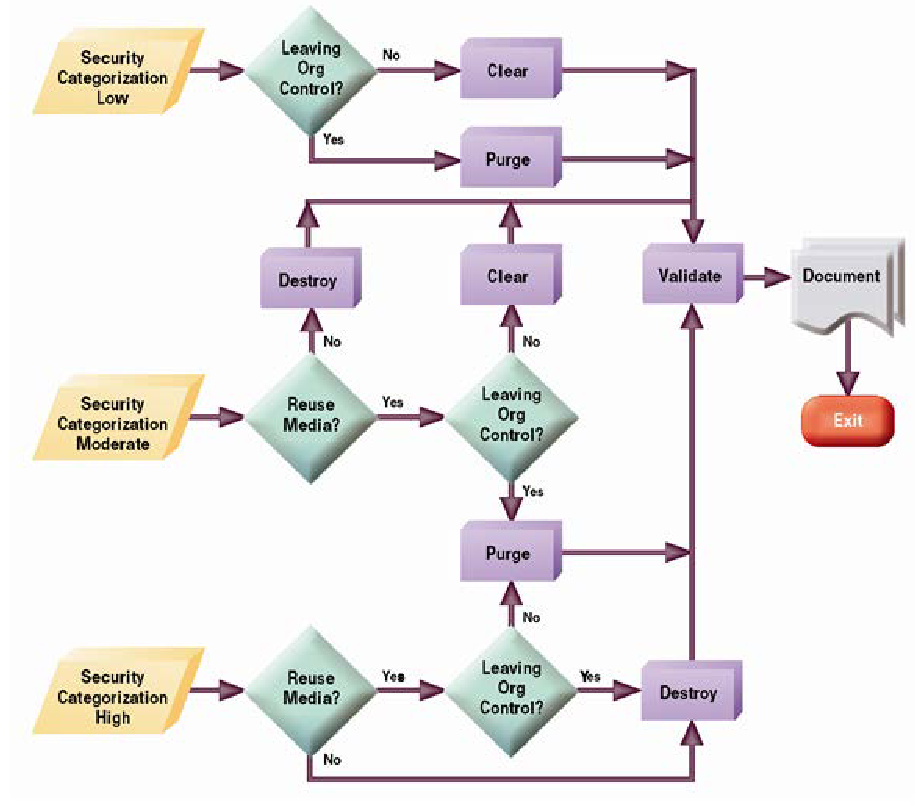
\includegraphics[height=2.5in]{screen1.png} \\

\vspace{\baselineskip}
\scriptsize \textbf{Source:} \href{https://nvlpubs.nist.gov/nistpubs/SpecialPublications/NIST.SP.800-88r1.pdf}{NIST SP 800-88R1 --- Guidelines for Media Sanitization, National Institute of Standards and Technology, US}
\end{frame}

\begin{frame}{PIPEDA -- 6. Accuracy}
\begin{itemize}
   \item Ensure accuracy, completeness, and currency of information
   \item Record collection dates for all information
   \item Record and document measures for ensuring accuracy
\end{itemize}

\vspace{\baselineskip}
\scriptsize \textbf{Source:} \href{https://www.priv.gc.ca/en/privacy-topics/privacy-laws-in-canada/the-personal-information-protection-and-electronic-documents-act-pipeda/p_principle/principles/p_accuracy/}{PIPEDA Fair Information Principle 6 -- Accuracy (OPC)} 
\end{frame}

\begin{frame}{PIPEDA -- 6. Accuracy \small (Interpretation)}
\begin{itemize}
   \item Information must be as accurate as necessary for purpose
   \item Industry standards are not an appropriate reference for adequate accuracy
   \item Responsibility for accuracy rests with the organization, not the individual
   \item Information must be updated also to third parties
\end{itemize}

\vspace{\baselineskip}
\scriptsize \textbf{Source:} \href{https://www.priv.gc.ca/en/privacy-topics/privacy-laws-in-canada/the-personal-information-protection-and-electronic-documents-act-pipeda/pipeda-compliance-help/pipeda-interpretation-bulletins/interpretations_04_accuracy/}{Interpretation Bulletin: Accuracy (OPC)}
\end{frame}

\begin{frame}{PIPEDA -- 7. Safeguards}
\begin{itemize}
   \item Develop and implement security policies
   \item Use physical, technological, and organizational measues to provide protection
   \item Anonymize unnecessary personal information
   \item Review safeguards
   \item Employee training and education
\end{itemize}

\vspace{\baselineskip}
\scriptsize \textbf{Source:} \href{https://www.priv.gc.ca/en/privacy-topics/privacy-laws-in-canada/the-personal-information-protection-and-electronic-documents-act-pipeda/p_principle/principles/p_safeguards/}{PIPEDA Fair Information Principle 7 -- Safeguards (OPC)}
\end{frame}

\begin{frame}{PIPEDA -- 7. Safeguards \small (Interpretation)}
\begin{itemize}
   \item Safeguards must be commensurate with sensitivity
   \item Policies must be effectively applied
   \item Secure disposal policies must be implemented
   \item Medical and payroll information are highly sensitive
   \item Employee training and education is required
   \item Organizations must ensure that third parties have safeguards in place
   \item Data on portable devices must be encrypted
   \item Data in online storage must be encrypted
   \item Organizations must ensure technological safeguards remain current
\end{itemize}

\vspace{\baselineskip}
\scriptsize \textbf{Source:} \href{https://www.priv.gc.ca/en/privacy-topics/privacy-laws-in-canada/the-personal-information-protection-and-electronic-documents-act-pipeda/pipeda-compliance-help/pipeda-interpretation-bulletins/interpretations_08_sg/}{Interpretation Bulletin: Safeguards (OPC)}
\end{frame}

\begin{frame}{PIPEDA -- 7. Safeguards \small (''Employee Snooping'')}
\begin{itemize}
   \item Privacy culture
   \item Training and reminders
   \item Policies for granting and revoking access
   \item Ensure access is restricted to roles, geography, time, etc.
   \item Monitor access and detect anomalies and inappropriate access
\end{itemize}

\vspace{\baselineskip}
\scriptsize \textbf{Source:} \href{https://www.priv.gc.ca/en/privacy-topics/business-privacy/safeguards-and-breaches/privacy-breaches/02_05_d_65_tips/}{Ten tips for addressing employee snooping (OPC)}
\end{frame}

\begin{frame}{PIPEDA -- 8. Openness}
\begin{itemize}
  \item Inform customers and employees about policies and procedures
  \item Ensure that policies are easily available and easy to understandable
  \item Specify (at minimum):
  \begin{itemize}
     \item Accountable person 
     \item How to access and amend/update/delete personal information
     \item How to complain about practices
     \item Collected information and disclosure to others
  \end{itemize}
\end{itemize}

\vspace{\baselineskip}
\scriptsize \textbf{Source:} \href{https://www.priv.gc.ca/en/privacy-topics/privacy-laws-in-canada/the-personal-information-protection-and-electronic-documents-act-pipeda/p_principle/principles/p_openness/}{PIPEDA Fair Information Principle 8 -- Openness (OPC)}
\end{frame}

\begin{frame}{Hands-On Exercise}
\begin{columns}
\begin{column}{0.2\textwidth}
\href{https://commons.wikimedia.org/wiki/File:Emojione_BW_1F44B.svg}{
\includegraphics[width=\textwidth]{hand.png}}
\end{column}
\begin{column}{0.8\textwidth}

Consider your bank or communications provider or other large organization you regularly deal with. 
\begin{itemize}
  \item What policies or procedures do they communicate?
  \item Where can you find them? Are they easy to find? Are they easy to understand?
\end{itemize}
\end{column}
\end{columns}
\end{frame}

\begin{frame}{PIPEDA -- 9. Individual Access}
\begin{itemize}
   \item Advise individuals about their information held, how it was collected and used, and disclosures to third parties. 
   \item Requests have to be in writing
   \item Verify requestor identify before disclosing to requestor
   \item Document requests for information and their processing, incl. the documents provided to the requestor
   \item Provide access at minimal or no cost, using easy process
%   \item Notify requestor of approximate cost and confirm they are willing to proceed
   \item 30 day to provide requested information; 30 day extension in exceptional circumstances (e.g. legal consult, format shifting, etc.)
   \item Ensure retention is updated
   \item Inform individuals of their right to complain to OPC
   \item Ensure staff training
\end{itemize}

\vspace{\baselineskip}
\scriptsize \textbf{Source:} \href{https://www.priv.gc.ca/en/privacy-topics/privacy-laws-in-canada/the-personal-information-protection-and-electronic-documents-act-pipeda/p_principle/principles/p_access/}{PIPEDA Fair Information Principle 9 -- Individual Access (OPC)}
\end{frame}

\begin{frame}{PIPEDA -- 9. Access \small (Exemptions)}
\begin{itemize}
   \item Disclosure would reveal information about others
   \item Solicitor-client privilege
   \item Confidential commercial information
   \item Threaten security of others
\end{itemize}

\vspace{\baselineskip}
\scriptsize \textbf{Source:} \href{https://www.priv.gc.ca/en/privacy-topics/accessing-personal-information/obligations-for-organizations/02_05_d_54_ati_02/}{Responding to access to information requests under PIPEDA (OPC)}
\end{frame}

\begin{frame}{Hands-On Exercise}
\begin{columns}
\begin{column}{0.2\textwidth}
\href{https://commons.wikimedia.org/wiki/File:Emojione_BW_1F44B.svg}{
\includegraphics[width=\textwidth]{hand.png}}
\end{column}
\begin{column}{0.8\textwidth}
Consider your bank or communications provider or other large organization you regularly deal with. 
\begin{itemize}
  \item What is the process to access the information held about you? Who do you contact?
  \item Is access free or does it have an associated cost?
  \item What is the process to update your information? Who do you contact?
\end{itemize}
\end{column}
\end{columns}
\end{frame}

\begin{frame}{PIPEDA -- 10. Challenging Compliance}
\begin{itemize}
   \item Simple complaint handling procedures
   \item Inform complainants about organization's procedures, and those of industry bodies, regulators, and OPC
   \item Record and acknowledge complaints
   \item Notify and record outcomes, decisions, and actions taken in response
\end{itemize}

\vspace{\baselineskip}
\scriptsize \textbf{Source:} \href{https://www.priv.gc.ca/en/privacy-topics/privacy-laws-in-canada/the-personal-information-protection-and-electronic-documents-act-pipeda/p_principle/principles/p_compliance/}{PIPEDA Fair Information Principle 10 -- Challenging Compliance (OPC)}
\end{frame}   


\begin{frame}{Hands-On Exercise}
\begin{columns}
\begin{column}{0.2\textwidth}
\href{https://commons.wikimedia.org/wiki/File:Emojione_BW_1F44B.svg}{
\includegraphics[width=\textwidth]{hand.png}}
\end{column}
\begin{column}{0.8\textwidth}

Consider your bank or communications provider or other large organization you regularly deal with. 
\begin{itemize}
  \item How do you initiate a complaint about lack of compliance?
  \item Who do you contact?
\end{itemize}
\end{column}
\end{columns}
\end{frame}

   
\begin{frame}{PIPEDA -- Privacy Breach}
\begin{itemize}
   \item Report breaches of security safeguards that pose a real risk of significant harm to OPC
   \begin{itemize}
      \item Examples: Financial loss, identity theft, credit record, loss of employement or business opportunities, damage to reputation or relationships, damage to or loss of property, bodily harm
      \item Consider sensitivity of information
      \item Consider probability of misuse
   \end{itemize}
   \item Notify affected parties and third parties
   \item Maintain records of all breaches
   \item Responsibility to report for third party processor breaches
\end{itemize}

\vspace{\baselineskip}
\scriptsize \textbf{Source:} \href{https://www.priv.gc.ca/en/privacy-topics/business-privacy/safeguards-and-breaches/privacy-breaches/respond-to-a-privacy-breach-at-your-business/gd_pb_201810/}{What you need to know about mandatory reporting of breaches of security safeguards (OPC)}
\end{frame}

\begin{frame}{Other Data Protection and Privacy Laws}
\begin{itemize}
   \item European Union (GDPR)
   \item California (CCPA)
   \item US (COPPA, HIPAA)
   \item China (PIPL)
   \item Singapore (PDPA)
   \item South Africa (PoPIA)
   \item \ldots
\end{itemize}
\end{frame}


\begin{frame}{Bill C-27}
\begin{block}{Digital Charter Implementation Act 2022}
\begin{itemize}
   \item Consumer Privacy Protection Act (update to PIPEDA)
   \item Personal Information and Data Protection Tribunal Act
   \item Artificial Intelligence and Data Act (AIDA)
\end{itemize}
\end{block}
\begin{block}{Progress in House of Commons}
\begin{itemize}
   \item Minister for Innovation, Science and Economic Development
   \item First reading June 2022, second reading June 2023
   \item Standing Committee on Industry and Technology (in progress)
\end{itemize}
\end{block}

\begin{block}{Sources and Further Information}
\begin{itemize}
\item \href{https://www.parl.ca/legisinfo/en/bill/44-1/c-27}{Parliament of Canada}
\item \href{https://ised-isde.canada.ca/site/innovation-better-canada/en/artificial-intelligence-and-data-act-aida-companion-document}{AIDA Companion Document (Government of Canada)}
\end{itemize}
\end{block}
\end{frame}

\begin{frame}{AIDA}
  \begin{itemize}
     \item Prohibit reckless and malicious use of AI
     \item Ensure accountability of risks associated with AI systems
     \item Applicable to ''high-impact AI systems''
     \begin{itemize} 
        \item Severity of potential harm
        \item Evidence of risks to health or safety, risk of adverse impact on human rights
        \item Imbalances of economic and social circumstances, or age of impacted persons
        \item Consider both intended and unintended consequences
     \end{itemize}
  \end{itemize}
  
\vspace{\baselineskip}
  \begin{quote}''Artificial intelligence system means a technological system that, autonomously or partly autonomously, processes data related to human activities through the use of a genetic algorithm, a neural network, machine learning or another technique in order to generate content or make decisions, recommendations or predictions.''\end{quote} \scriptsize \href{https://www.parl.ca/legisinfo/en/bill/44-1/c-27}{Parliament of Canada}

\end{frame}

\begin{frame}{AIDA -- High Impact Examples}
  \begin{block}{Screening systems}
  \begin{itemize}
     \item Systems that make decisions, recommendations, or predictions
     \item Impacting access to services (e.g. credit) or employment
     \item Potential of discriminatory outcomes and economic harm
  \end{itemize}
  \end{block}
  
  \begin{block}{Biometric systems}
  \begin{itemize}
     \item Make predictions about people
     \item Identify person remotely
     \item Predict characteristics, psychology or behaviour
     \item Potential impact on mental health and autonomy
  \end{itemize}
  \end{block}
\end{frame}

\begin{frame}{AIDA -- High Impact Examples}
  \begin{block}{Influence human behaviour at scale}
  \begin{itemize}
     \item Content recommendation systems
     \item Influence behaviour, expression, and emotion
     \item Potential impact on psychological and physical health
  \end{itemize}
  \end{block}
  
  \begin{block}{Critical to health and safety}
  \begin{itemize}
     \item AI applications integrated in health and safety functions
     \item Decisions or recommendations based on sensor data
     \item Example: Autonomous driving systems
     \item Example: Triage decisions in health care
     \item Potential to cause physical harm
  \end{itemize}
  \end{block}
\end{frame}

\begin{frame}{AIDA -- Harms}
\begin{itemize}
  \item Individual harms
  \item Collective harms 
  \begin{itemize}
     \item Historically marginalized communities
     \item Human rights impacts
  \end{itemize}
  \item Biased output
  \begin{itemize}
     \item Differentiation directly or indirectly through variables that act as a proxy for prohibited grounds
     \item Race, gender, but also income (proxy for race or gender)
  \end{itemize}
  
  \vspace{\baselineskip}
  \begin{quote}''Biased output means content that is generated, or a decision, recommendation or prediction that is made, by an artificial intelligence system and that adversely differentiates, directly or indirectly and without justification, in relation to an individual on one or more of the prohibited grounds of discrimination set out in section 3 of the Canadian Human Rights Act \ldots''\end{quote}  \scriptsize \href{https://www.parl.ca/legisinfo/en/bill/44-1/c-27}{Parliament of Canada}
\end{itemize}
\end{frame}

\begin{frame}{AIDA -- Requirements}
\begin{block}{Human Oversight \& Monitoring}
\begin{itemize}
   \item Exercise meaningful human oversight
   \item Includes interpretability appropriate to context
   \item Measurement and assessment of high-impact AI systems and their output
\end{itemize}
\end{block}

\begin{block}{Transparency}
\begin{itemize}
   \item Publicly provide information on how high-impact AI is used
   \item Allow public to understand capabilities, limitations, and potential impacts
\end{itemize}
\end{block}
\end{frame}

\begin{frame}{AIDA -- Requirements}
\begin{block}{Fairness and Equity}
\begin{itemize}
   \item Demonstrate awareness of potential discriminatory outcomes
   \item Actions to mitigate discriminatory outcomes
\end{itemize}
\end{block}

\begin{block}{Safety}
\begin{itemize}
  \item Proactively assess high-impact AI systems to identify potential harms
  \item Mitigate risk of harm
\end{itemize}
\end{block}
\end{frame}

\begin{frame}{AIDA -- Requirements}
\begin{block}{Accountability}
\begin{itemize}
  \item Implement governance mechanisms to ensure compliance with AIDA
  \item Documentation of policies, processes, and implemented measures
\end{itemize}
\end{block}

\begin{block}{Validity \& Robustness}
\begin{itemize}
  \item Perform consistently with intended objectives
  \item Stable and resilient in a variety of circumstances
\end{itemize}
\end{block}
\end{frame}

\begin{frame}{AIDA -- Examples Measures}
\begin{block}{System Design}
\begin{itemize}
   \item Perform initial risk assessment
   \item Assess and address potential biases in training data selection
   \item System design informed by required level of interpretability
\end{itemize}
\end{block}

\begin{block}{System Development}
\begin{itemize}
   \item Document data and models
   \item Evaluate and validate, retrain as needed
   \item Build mechanisms for human oversight and monitoring
   \item Document appropriate use and limitations
\end{itemize}
\end{block}
\end{frame}

\begin{frame}{AIDA -- Examples Measures}
\begin{block}{Make System Available for Use}
\begin{itemize}
   \item Document how requirements for design and development are met
   \item Provide documentation to users regarding training data, limitations, and appropriate uses
   \item Continuous risk assessment
\end{itemize}
\end{block}

\begin{block}{Managing Operations of a System}
\begin{itemize}
   \item Logging and monitoring of output
   \item Ensure adequate monitoring and human oversight
   \item Intervene as needed
\end{itemize}
\end{block}
\end{frame}

\begin{frame}{AIDA}
\begin{itemize}
   \item Notification requirement in case of harm or potential material harm
   \item Specific requirements to be set through regulation by the Minister (expected within 2 years after royal assent)
   \item Minister would have power to audit, order cessation of use
\end{itemize}

\begin{block}{Enforcement Mechanisms}
\begin{itemize}
   \item Administrative monetrary penalties
   \item Regulary offences
   \item Criminal offences
\end{itemize}
\end{block}
\end{frame}

\begin{frame}{AIDA}
  \begin{block}{New Criminal Offences:}
   \begin{itemize}
      \item Knowingly possessing or using unlawfully obtained personal information to design, develope, use or make available for use an AI system.
      \item Making an AI system available for use, knowing, or being reckless as to whether it is likely to cause serious harm \ldots where its use actually causes such harm.
      \item Making an AI system available for use iwht the intent to defraud the public and to cause substantial economic loss to an individual, where its use actually causes that loss.
   \end{itemize}
\end{block}
\end{frame}

\begin{frame}{European Union AI Act}
\begin{block}{Source and Further Information}
\begin{itemize}
\item \href{https://www.europarl.europa.eu/topics/en/article/20230601STO93804/eu-ai-act-first-regulation-on-artificial-intelligence}{EU AI Act (European Parliament)}
\end{itemize}
\end{block}

\vspace{\baselineskip}
\centering
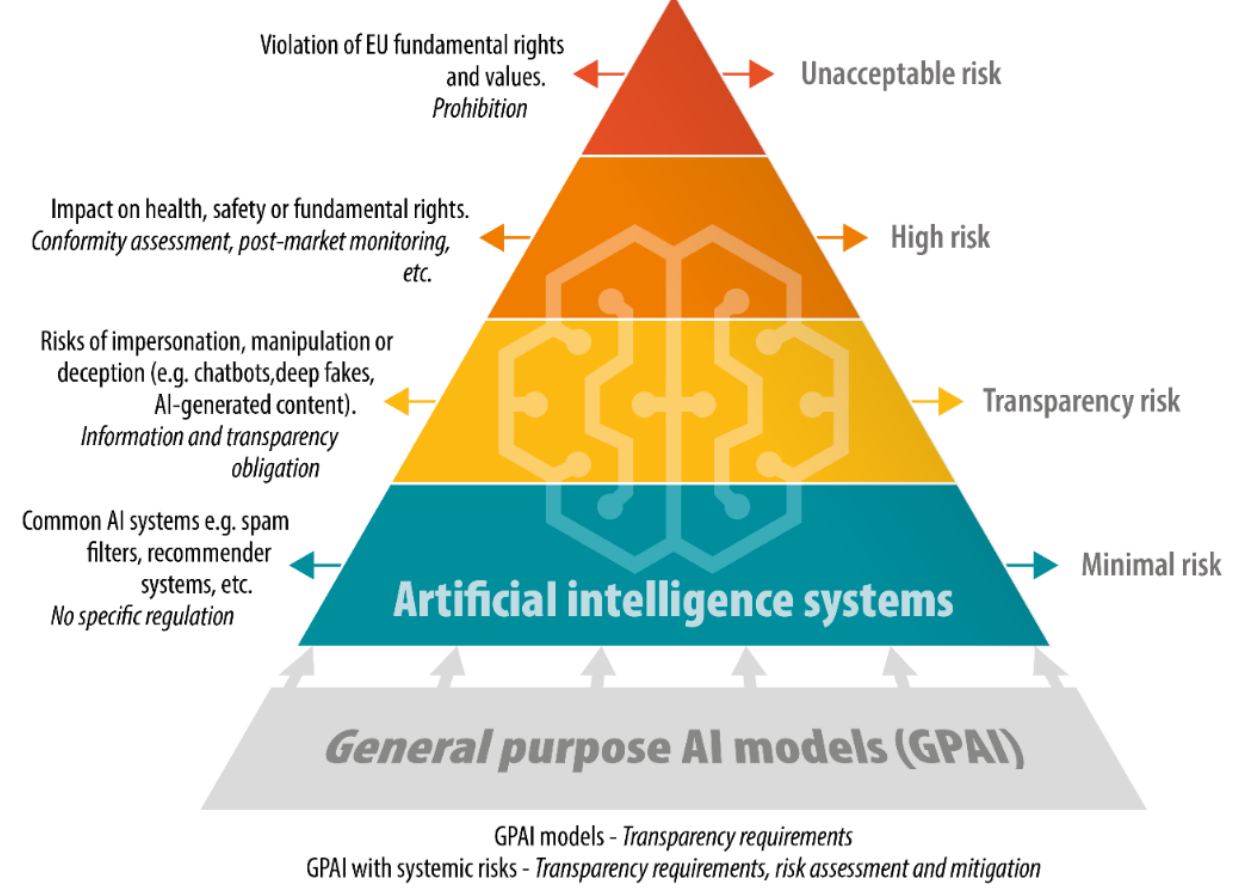
\includegraphics[height=2in]{screen2.png}

\vspace{\baselineskip}
\scriptsize \textbf{Source:} \href{https://www.europarl.europa.eu/RegData/etudes/BRIE/2021/698792/EPRS_BRI(2021)698792_EN.pdf}{AI Act Briefing (EU Parliament)}
\end{frame}


\begin{frame}{European Union AI Act}
\begin{block}{Unacceptable Risk}
\begin{itemize}
  \item Prohibited
  \item Examples:
	\begin{itemize}
	   \item Cognitive behavioural manipulation
	   \item Classifying people based on behaviour, socio-economic status or personal characteristics (''social scoring'')
	   \item Untargeted scraping of internet for facial images 
	   \item Emotion recognition in the workplace and educational institutions (except for medical or safety reasons)
	   \item Biometric categorisation to infer race, sexual orientation, political opinions, religous beliefs
	   \item Real-time remote biometric identification systems in public spaces, such as facial recognition
	\end{itemize}
\end{itemize}
\end{block}
\end{frame}

\begin{frame}{European Union AI Act}
\begin{block}{High Risk}
\begin{itemize}
   \item Asssessment before market introduction and throughout product lifecycle
   \item AI systems that are used in products are subject to EU product safety legislation (e.g. toys, aircraft, cars, medical devices, etc.)
   \item Profiling of natural persons
   \item Registration requirement for specific areas:
	\begin{itemize}
	  \item Operation of critical infrastructure
	  \item Education and vocational training
	  \item Employment, worker management and access to self-employment
	  \item Access to essential private and public services, \& benefits
	  \item Law enforcement
	  \item Migration, asylum, and border control
	  \item Assistance in legal interpretation and application of the law
    \end{itemize}
\end{itemize}
\end{block}
\end{frame}

\begin{frame}{European Union AI Act}
\begin{block}{Transparency Risk}
\begin{itemize}
   \item Risk of impersonation, manipulation, or deception
   \item Chatbots, deep fakes, AI-generated content, \ldots
   \item Information and transparency obligation
   \item E.g. watermarking output, disclosure of AI generated content
\end{itemize}
\end{block}

\begin{block}{Minimal Risk}
\begin{itemize}
   \item Common AI systems
   \item No specific regulation
\end{itemize}
\end{block}
\end{frame}

\end{document}
